\section{Beberapa Kelas Gelanggang Khusus}
Misalkan $R$ gelanggang; sepanjang bagian ini kita mengandaikan bahwa $R$ tak nol. Untuk setiap $x \in R$, definisikan \emph{sentralisator}-nya
\[ Z_R(x) := \left\{ r \in R : rx=xr \right\}; \]
\emph{Pusat} gelanggang $R$ didefinisikan sebagai\index{zhongxin@pusat}\index[sym1]{$Z_R$}
\[ Z_R := \left\{r \in R : \forall s \in R, rs=sr \right\} = \bigcap_{x \in R} Z_R(x). \]
Semua himpunan ini merupakan subgelanggang dari $R$, dan $Z_R$ merupakan gelanggang komutatif.

Karena $R$ membentuk monoid terhadap perkalian, invers kiri dan invers kanan bagi unsur-unsurnya dapat didefinisikan. Misalkan $r \in R$ tak nol. Jika $r$ invertibel, inversnya ditulis $r^{-1}$; grup perkalian semua unsur invertibel ditulis $R^\times$. Jika terdapat $r' \neq 0$ sedemikian sehingga $rr'=0$, maka $r$ disebut \emph{pembagi nol kiri}; jika syaratnya diganti menjadi $r'r=0$, maka disebut \emph{pembagi nol kanan}. Unsur-unsur di $R$ yang merupakan pembagi nol kiri atau kanan secara kolektif disebut \emph{pembagi nol}. Unsur $r \in R \smallsetminus \{0\}$ bukan pembagi nol kiri jika dan hanya jika perkalian kiri oleh $r$ memenuhi hukum pencoretan, sebab $ra=rb \iff r(a-b)=0$; kasus pembagi nol kanan serupa.\index{lingyinzi@pembagi nol (zero divisor)}

Karena gelanggang membentuk grup terhadap penjumlahan, setiap unsurnya dapat dikalikan dengan sebarang bilangan bulat: misalnya $(-1)r = -r$, $nr = \underbracket{r + \cdots + r}_{n\; \text{suku}}$, $(-n)r = -nr$, dan seterusnya (dengan $n \geq 0$). Mudah diperiksa bahwa pemetaan
\begin{equation}\label{eqn:ring-struct-morphism}\begin{aligned}
	\Z & \longrightarrow R \\
	a & \longmapsto a \cdot 1_R
\end{aligned}\end{equation}
merupakan homomorfisme gelanggang; ini juga merupakan satu-satunya homomorfisme dari $\Z$ ke $R$, dan citranya termuat di dalam $Z_R$. Menurut Proposisi \ref{prop:1st-homomorphism-ring} dan Contoh \ref{eg:Z-pid}, citranya niscaya isomorfik dengan suatu $\Z/p\Z$, dengan $p \in \Z_{\geq 0}$ yang unik. Di sini harus berlaku $p \neq 1$, sebab jika tidak, di dalam $R$ persamaan $1=0$ akan mengakibatkan $R$ menjadi gelanggang nol. Bilangan $p$ ini ditulis $\text{char}(R)$.

\begin{definition}\label{def:ring-characteristic}\index{tezheng@karakteristik (characteristic)}\index[sym1]{char@$\text{char}(R)$}
	Misalkan $R$ gelanggang tak nol. \emph{Karakteristiknya} didefinisikan sebagai $\text{char}(R)$ di atas.
\end{definition}
Jika $R$ tidak mempunyai pembagi nol tak nol, maka $\Z/p\Z$ juga demikian; kondisi terakhir berlaku jika dan hanya jika $p=0$ atau bilangan prima. Rumus berikut khususnya berguna dalam teori medan: misalkan gelanggang komutatif $R$ berkarakteristik bilangan prima $p$, maka
\begin{equation}\label{eqn:freshmen-dream}
	(u+v)^{p^m} = u^{p^m} + v^{p^m}, \quad u, v \in R, \; m \geq 0;
\end{equation}
ini merupakan penerapan langsung teorema binomial atas $R$ dan Lema \ref{prop:Wielandt-lemma}.

\begin{definition}\index{zhenghuan@daerah integral (integral domain)}
	Gelanggang komutatif tanpa pembagi nol tak nol disebut \emph{daerah integral}.
\end{definition}

\begin{definition}\label{def:field}\index{chuhuan@gelanggang pembagian (division ring)}\index{yu@medan (field)}
	Jika setiap unsur tak nol di gelanggang $R$ invertibel, maka $R$ disebut \emph{gelanggang pembagian}. Gelanggang pembagian yang komutatif disebut \emph{medan}.
\end{definition}
Menurut konvensi bagian ini, gelanggang pembagian tidak boleh merupakan gelanggang nol; dalam sebagian literatur, gelanggang pembagian disebut juga medan miring.

\begin{example} \index[sym1]{F_q@$\F_q$}
	Misalkan $p$ bilangan prima. Gelanggang hasil bagi $\Z/p\Z$ adalah medan, yang biasanya ditulis $\F_p$. Memang, jika $x \in \Z$ relatif prima dengan $p$, algoritma Euclid memperlihatkan bahwa $xy + pz = 1$ mempunyai solusi bilangan bulat $y,z$; karena itu $y+p\Z$ memberikan invers perkalian bagi $x+p\Z$.
\end{example}
Di dalam gelanggang pembagian $D$ pembagian dapat dilakukan, sehingga terdapat submedan terkecil yang memuat $1$, yang disebut \emph{submedan prima} dari $D$; jika $\text{char}(D)=0$, maka $\Z \hookrightarrow D$, sehingga submedan primanya isomorfik dengan medan bilangan rasional $\Q$; jika $\text{char}(D)=p > 0$, submedan primanya adalah $\F_p$ di atas. \index{suziyu@submedan prima (prime subfield)}

Syarat topologis, struktur geometris, atau kondisi keterhinggaan pada suatu gelanggang sering berhubungan secara halus dengan sifat-sifat aljabarnya. Kedua hasil berikut merupakan contoh yang sangat baik. Bukti Teorema \ref{prop:Wedderburn-little-thm} memerlukan sedikit pengetahuan tentang polinomial dan teori bilangan elementer.

\begin{proposition}
	Jika gelanggang hingga $D$ tidak mempunyai pembagi nol tak nol, maka $D$ merupakan gelanggang pembagian.
\end{proposition}
\begin{proof}
	Misalkan $x \in D$, $x \neq 0$. Berdasarkan hipotesis, pemetaan dari $D$ ke dirinya sendiri yang diberikan oleh perkalian kiri $L_x: r \mapsto xr$ bersifat injektif. Karena $D$ hingga, $L_x$ otomatis bijektif, sehingga terdapat $x' \in D$ sedemikian sehingga $xx'=1$, yakni $x$ mempunyai invers kanan. Demikian pula, dengan meninjau pemetaan perkalian kanan, diperoleh bahwa $x$ mempunyai invers kiri. Karena itu $x \in D^\times$.
\end{proof}

\begin{theorem}[Teorema Kecil Wedderburn]\label{prop:Wedderburn-little-thm}\index{Wedderburn@Teorema Kecil Wedderburn}
	Setiap gelanggang pembagian hingga merupakan medan.
\end{theorem}
\begin{proof}[E.\ Witt]
	Misalkan $D$ gelanggang pembagian hingga. Untuk setiap $r \in D^\times$, dengan menerapkan aksi konjugasi oleh $r^{\pm 1}$ pada $D$, diperoleh bahwa untuk setiap $x \in D$,
	\[ xr = rx \iff r^{-1}x = xr^{-1}. \]
	Dari sini diperoleh dua konsekuensi. Pertama, $Z_D(x) \smallsetminus \{0\}$ tertutup terhadap pengambilan invers, sehingga $Z_D(x)$ merupakan subgelanggang pembagian. Kedua, $Z_D \smallsetminus \{0\}$ juga tertutup terhadap pengambilan invers, sehingga $Z_D$ merupakan medan. Selanjutnya, tetapkan $F := Z_D$ dan tuliskan kardinalitasnya sebagai $q \in \Z_{\geq 2}$.

	Perhatikan bahwa gelanggang $D$, melalui perkalian oleh $F$, membentuk ruang vektor atas $F$; menurut hipotesis, $n := \dim_F D$ berhingga. Di bawah ini akan dibuktikan bahwa $n = 1$, dan dari sini segera diperoleh bahwa $D = F$ komutatif.

	Untuk aksi konjugasi dari grup perkalian $D^\times = D \smallsetminus \{0\}$, penerapan Lema \ref{prop:orbit-decomp} memberikan
	\begin{equation}\label{eqn:Wedderburn-little}
		q^n - 1 = \underbracket{q-1}_{= |F^\times|} + \sum_x (D^\times : Z_D(x)^\times)
	\end{equation}
	di mana $x$ menjelajahi suatu himpunan wakil bagi $D^\times \smallsetminus F^\times$ di bawah aksi konjugasi. Perhatikan bahwa $Z_D(x)$ juga merupakan ruang vektor atas $F$; tuliskan dimensinya sebagai $n(x) \in \Z_{\geq 1}$. Dengan demikian, $n(x) < n$ dan
	\[ (D^\times : Z_D(x)^\times) = \dfrac{q^n - 1}{q^{n(x)} - 1}. \]
	Kami menegaskan bahwa $n(x) \mid n$. Berdasarkan hasil teori bilangan elementer atau Contoh \ref{eg:gcd-cyclotomic} yang akan muncul kemudian, faktor persekutuan terbesar dari $q^n - 1$ dan $q^{n(x)} - 1$ adalah $q^{(n, n(x))} - 1$. Karena itu, $\frac{q^n - 1}{q^{n(x)} - 1} = (D^\times : Z_D(x)^\times) \in \Z$ mengakibatkan $n(x) \mid n$, sebagaimana dikehendaki. Cara lain ialah memandang $D$ sebagai ruang vektor kiri atas gelanggang pembagian $Z_D(x)$; dalam hal itu $n/n(x) = \dim_{Z_D(x)} D$. Cara ini memerlukan teori dari \S\ref{sec:vector-space} dan diserahkan kepada pembaca untuk ditelaah.
	
	Sekarang kita akan menerapkan teori polinomial siklotomik. Ini adalah keluarga polinomial berkoefisien bilangan bulat dengan koefisien terdepan $1$ (disingkat monik), yaitu $\Phi_r(X)$, $r \in \Z_{\geq 1}$, sedemikian sehingga\index{fenyuanduoxiangshi@polinomial siklotomik (cyclotomic polynomial)}
	\begin{gather*}
		X^m - 1 = \prod_{r \mid m} \Phi_r(X), \quad m \in \Z_{\geq 1}, \\
		\deg \Phi_r = \varphi(r) := |(\Z/r\Z)^\times| \qquad \text{(fungsi Euler)}
	\end{gather*}
	selalu berlaku. Definisi langsungnya ialah
	\begin{align*}
		\Phi_m(X) & = (X^m - 1) \cdot \prod_{\substack{p: \text{prima} \\ p \mid m}} (X^{m/p} - 1)^{-1} \cdot \prod_{\substack{p \neq q: \text{prima} \\ pq \mid m}} (X^{m/pq} - 1) \cdots \\
		& = \prod_{d \mid m} (X^d - 1)^{\mu(m/d)}, \\
		\deg \Phi_m & = \sum_{d \mid m} d \mu\left( \frac{m}{d} \right) = \sum_{h \mid m} \frac{m}{h} \cdot \mu(h) \\
		& = \varphi(m) \qquad \because \text{teori bilangan elementer, atau \eqref{eqn:Euler-phi-sum}};
	\end{align*}
	di mana $\mu$ menyatakan fungsi Möbius
	\[ \mu(d) = \begin{cases}
		(-1)^{(\text{banyaknya faktor prima dari }\; d)}, & d \;\text{tidak mempunyai faktor kuadrat selain $1$} \\
		0, & d \; \text{mempunyai faktor kuadrat} \neq 1.
	\end{cases}\]
	Karena di dalam gelanggang polinomial berkoefisien bilangan bulat, $X^{(a,b)}-1$ merupakan faktor persekutuan terbesar dari $X^a - 1$ dan $X^b - 1$ (Contoh \ref{eg:gcd-cyclotomic}), maka $\Phi_m(X)$ yang didefinisikan dengan cara ini memang merupakan polinomial monik berkoefisien bilangan bulat. Sebenarnya, polinomial ini adalah inti yang diperoleh dengan menerapkan prinsip inklusi-eksklusi untuk menyingkirkan dari $X^m - 1$ semua faktor monik yang berasal dari $X^d - 1$ ($d \mid m, d \neq m$). Kita akan membahas kerangka umum inversi Möbius dalam \S\ref{sec:Mobius}, lalu meninjau kembali versi klasik yang digunakan di sini dalam Contoh \ref{eg:Mobius-classical} (tepatnya, kasus ``multiplikatif''-nya). Kajian sistematis mengenai polinomial siklotomik merupakan tugas \S\ref{sec:cyclotomic-ext}.

	Di atas medan bilangan kompleks $\CC$, polinomial $\Phi_m(X)$ dapat difaktorkan sebagai $\prod_\zeta (X-\zeta)$, dengan $\zeta$ menjelajahi semua unsur di dalam $\CC^\times$ yang merupakan akar satuan ke-$m$ primitif. Karena $n(x) \mid n$ dan $n(x) < n$, kita memperoleh hubungan keterbagian antara polinomial-polinomial monik berkoefisien bilangan bulat
	\[ \Phi_n(X) \mid X^n - 1, \quad \Phi_n(X) \mid \prod_{\substack{d \mid n \\ d \nmid n(x)}} \Phi_d(X) = \frac{X^n - 1}{X^{n(x)} - 1}; \]
	Rumus di atas juga dapat dibuktikan melalui faktorisasi di atas $\CC$. Setelah menyubstitusikan $X \leadsto q \in \Z$, terlihat bahwa di dalam \eqref{eqn:Wedderburn-little}, $q^n-1$ dan setiap suku $\frac{q^n - 1}{q^{n(x)} - 1}$ semuanya habis dibagi $\Phi_n(q)$; oleh karena itu $\Phi_n(q)  \mid  q-1$. Di sisi lain, andaikan $n>1$. Maka, di dalam $\CC^\times$, untuk setiap akar satuan ke-$n$ yang primitif $\zeta$, berlaku
	\[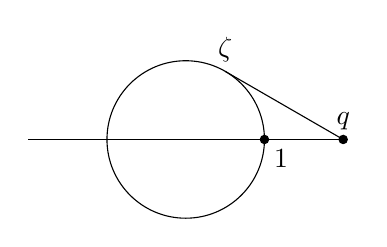
\begin{tikzpicture}[baseline=(O)]
		\draw (0,0) circle [radius=1cm];
		\draw (-2,0) -- (2,0);
		\coordinate (O) at (0:1cm); \coordinate (Q) at (2,0);  \coordinate (Z) at (60:1cm);
		\node[below right] at (O) {$1$}; \draw[fill=black] (O) circle [radius=1.5pt]; 
		\node[above] at (Q) {$q$}; \draw[fill=black] (Q) circle [radius=1.5pt];
		\node[above] at (Z) {$\zeta$};
		\draw (Q) -- (Z);
	\end{tikzpicture} \qquad
	\implies \quad |q-\zeta| > q-1 \geq 1.
	\]
	Jadi $|\Phi_n(q)| = \prod_\zeta |q-\zeta| > q-1$, yang menghasilkan kontradiksi.
\end{proof}

Gelanggang pembagian takkomutatif ditemukan cukup lambat; contoh paling awal yang dapat dilacak ialah temuan W.\ Hamilton pada 1843, yaitu \emph{aljabar kuaternion}. Kelak, ketika membahas aljabar berdimensi hingga, kita akan memberikan beberapa metode sistematis untuk membangun gelanggang pembagian semacam ini.
\begin{example}[Kuaternion]\label{eg:Hamilton-quaternion}\index{siyuanshu@kuaternion (quaternion)}\index[sym1]{H@$\mathbb{H}$}
	Tinjau ruang vektor real dengan basis $1, i, j, k$, yaitu $\mathbb{H} := \R 1 \oplus \R i \oplus \R j \oplus \R k$. Pada ruang ini terdapat perkalian yang terdefinisi dengan baik sehingga $\mathbb{H}$ menjadi gelanggang dan memenuhi sifat-sifat berikut:
	\begin{itemize}
		\item Perkalian $(x,y) \mapsto xy$ merupakan pemetaan bilinear pada $\mathbb{H}$;
		\item $1$ merupakan unsur satuan perkalian, sehingga kita dapat mengidentifikasi $\R$ dengan $\R \cdot 1$ dan membenamkannya ke dalam $Z_{\mathbb{H}}$;
		\item $i^2 = j^2 = -1$;
		\item $ij=k=-ji$.
	\end{itemize}
	Dari sini dapat diturunkan bahwa $k^2 = -1$, $jk=i=-kj$, dan $ki=j=-ik$. Rinciannya diserahkan kepada pembaca. Berdasarkan struktur ruang vektor dan kedua sifat pertama, kita juga menyebut $\mathbb{H}$ sebagai suatu ``$\R$-aljabar''; Definisi \ref{def:algebra-naive} akan memberikan penjelasan terperinci. Selain itu, medan bilangan kompleks $\CC = \R \oplus \R i$ dapat dibenamkan ke dalam $\mathbb{H}$. Berikut ini kita periksa bahwa $\mathbb{H}$ merupakan gelanggang pembagian. Jika operasi konjugasi didefinisikan oleh
	\[ z = a + bi + cj + dk \longmapsto \bar{z} = a - bi -cj -dk \]
	maka berlaku $\overline{z w} = \bar{w}\bar{z}$ dan $z\bar{z} = \bar{z}z = a^2 + b^2 + c^2 + d^2 \in \R$; dari sini diperoleh
	\[ z^{-1} = (z\bar{z})^{-1} \bar{z} = (\underbracket{a^2 + b^2 + c^2 + d^2}_{\neq 0})^{-1} \bar{z}, \quad z \in \mathbb{H} \smallsetminus \{0\}. \]
	Sifat kunci yang digunakan di sini dapat dikembalikan pada fakta bahwa $a^2 + b^2 + c^2 = -1$ tidak mempunyai solusi di dalam medan bilangan real $\R$. Pernyataan yang lebih kuat ialah bahwa $-1$ bukan jumlah kuadrat di dalam $\R$; medan yang memenuhi kondisi terakhir disebut medan real formal, dan merupakan objek yang sangat menarik dalam kajian teori medan, bentuk kuadratik, serta teori model; lihat \cite[\S 9.1]{Feng17}. \index{moxinglun@teori model}
\end{example}
